\section*{Задание 2}

\subsection*{Задание}

При помощи графа де Брюина найдите все слова наименьшей длины,
которые содержат подстроки

$$ KQS, QSU, UQS, SQU, SUQ, QSQ, QUQ, UQU. $$

\subsection*{Решение}

Построим граф де Брюина:

\begin{figure}[H]
    \centering
    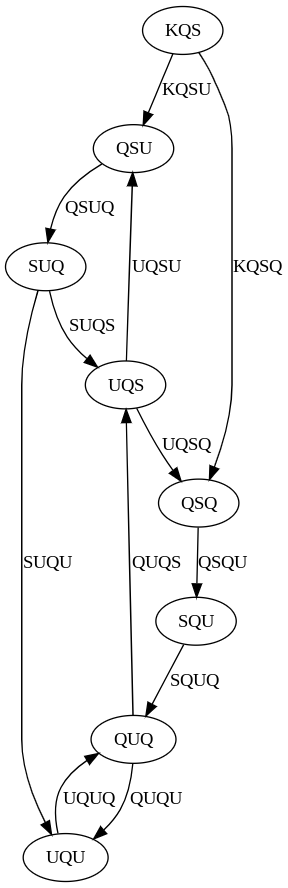
\includegraphics[width=0.28\linewidth]{photo/2s0}
    \caption{Граф де Брюина для подстрок $ KQS, QSU, UQS, SQU, SUQ, QSQ, QUQ, UQU $}
    \label{fig:2s0}
\end{figure}

Из рис.~\ref{fig:2s0} видно, что искомые слова (12):

KQSU,
KQSQ,
QSUQ,
UQSU,
UQSQ,
SQUQ,
SUQS,
SUQU,
QSQU,
QUQS,
QUQU,
UQUQ.
